\chapter{Box Registers}
 

Many applications of box registers can be found in the Chapters on output 
routines. 

There are 256 box registers, as is the case with all other register types. Box 
register 255 is reserved for a special purpose; in it \tex stores the current page 
before it ships the current page out to the dvi file. 
This register should only be used by the output routine, but not 
otherwise.
 
\begin{docCommand}{newbox}{\marg{\textbackslash boxname}}{}
There are no box parameters. Box registers 0-9 are reserved for temporary use, as is the case with registers 
in that register index range in general. 
\end{docCommand}

Allocating a New Box Register, |\newbox| 

A new box register can be allocated with |\newbox| as in |\newbox\abox|. Now 
|\abox| stands for the box register index allocated by |\newbox|. As usual the 
allocation of box registers using |\newbox| starts with register 10. 


If you assume that TeX allocated box register 16, then |\the\abox| prints 
16, the box register index, not the content of box register 16. The command 
|\the| cannot be used to print the content of a box register; you must use |\box| 
or |copy|instead.  

\begin{texexample}{Saving Material in a Box Register}{ex:boxregister}
\newbox\lenna %(*@\dcircle{1}@*)

\setbox\lenna=\vbox{% (*@\dcircle{2}@*)
 The width of the line \the\linewidth 
 \hsize=300pt\par\leavevmode
 \hbox{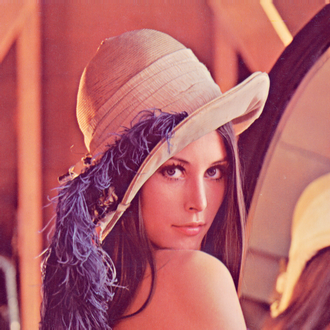
\includegraphics[width=100pt]{lenna}}%
 \hbox{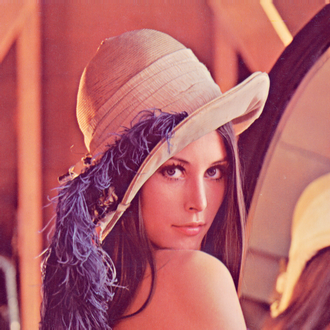
\includegraphics[width=100pt]{lenna}}%
 \hbox{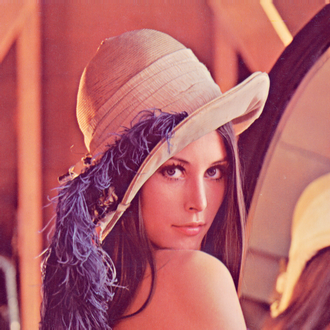
\includegraphics[width=100pt]{lenna}}%
}
\copy\lenna

%\copy\lenna
\the\ht\lenna\ The height of the box stored in box register\\
\the\dp\lenna\ The depth of the box stored in box register\\
\the\wd\lenna\ The width of the box stored in box register\\ 


\unvbox\lenna
\the\ht\lenna\ The height of the box stored in box register\\
\the\dp\lenna\ The depth of the box stored in box register\\
\the\wd\lenna\ The width of the box stored in box register\\ 

\end{texexample}

In the example we created a new box to hold the material at \dcircle{1}. Then we inserted the material using |\setbox| at \dcircle{2}. 

\section{Box Dimensions}

As we can observe from Example~\ref{ex:boxregister} the valus of the box dimensions can be printed using |\the|. Unfortunately \tex's rules does not allow us to change these dimensions directly using \tex's arithmetical commands such as |\advance|. In order to do this we need to store them in length registers first.

\begin{texexample}{Saving Material in a Box Register}{ex:boxregister}
\newbox\lenna %(*@\dcircle{1}@*)

\setbox\lenna=\vbox{% (*@\dcircle{2}@*)
 \hsize=300pt\par\leavevmode
 \hbox{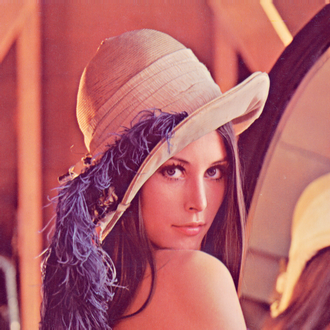
\includegraphics[width=100pt]{lenna}}%
 \hbox{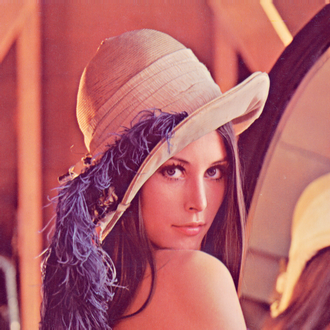
\includegraphics[width=100pt]{lenna}}%
 \hbox{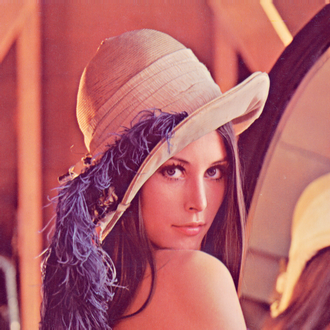
\includegraphics[width=100pt]{lenna}}%
}

\the\ht\lenna\ The height of the box stored in box register\\
\the\dp\lenna\ The depth of the box stored in box register\\
\the\wd\lenna\ The width of the box stored in box register\\ 

% use a scratch register
\newdimen\scratchdimen

% set it to the original \ht height
\scratchdimen=\ht\lenna

% set it to the original ht + 20pt
\advance\scratchdimen  by 20pt\relax

% add 10pt


\ht\lenna=\scratchdimen

\copy\lenna

\unvbox\lenna
\the\ht\lenna\ The height of the box stored in box register\\
\the\dp\lenna\ The depth of the box stored in box register\\
\the\wd\lenna\ The width of the box stored in box register\\ 
\end{texexample}

We can see that \tex did not change the dimensions of the box contents, but did change the size of the containing box (now we have a vertical space between the two sets of images). We could have changed the |wd| and |dp| as well. Since we are manipulating dimensions all of \latexe's macros for length can be used or we can buid our own.


Note that the dimensions of a void box register are zero, but a box with all dimensions 
are of zero length is not necessarily empty.  As seen in the last example, you can load a box register and then set all three dimensions to zero without affecting the contents of this register. 


\section{Using \latex2e Constructs}

As for the rest of the registers the LaTeX Team abstracted  some of the commands to different macros:

\begin{texexample}{test}{}
\newsavebox{\amato}

\savebox{\amato}{%
  \fbox{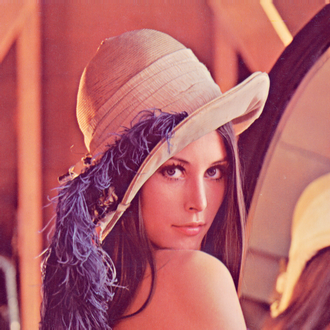
\includegraphics[width=100pt]{lenna}}%
 \fbox{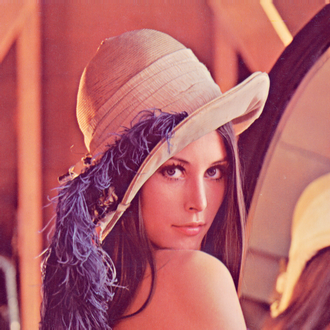
\includegraphics[width=100pt]{lenna}}%
 \fbox{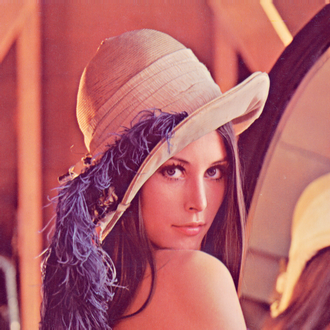
\includegraphics[width=100pt]{lenna}}%
 \parbox[b]{80pt}{\RaggedRight\bfseries Some caption text goes here}
}
\overfullrule3pt
\usebox\amato

\usebox\amato
\end{texexample}






\endinput